\documentclass[aspectratio=169,10pt]{beamer}

% ── Theme ─────────────────────────────────────────────────────────────────────
\usetheme{Madrid}
\usecolortheme{seahorse}
\setbeamertemplate{navigation symbols}{}
\setbeamertemplate{footline}[frame number]

% ── Packages ──────────────────────────────────────────────────────────────────
\usepackage{amsmath,amssymb}
\usepackage{booktabs}
\usepackage{tikz}
\usepackage{pgfplots}
\pgfplotsset{compat=1.17}
\usepackage{xcolor}
\usepackage{listings}
\usepackage{microtype}

% ── Colours ───────────────────────────────────────────────────────────────────
\definecolor{euroblue}{RGB}{31,119,180}
\definecolor{amred}{RGB}{214,39,40}
\definecolor{btgreen}{RGB}{44,160,44}
\definecolor{codegray}{RGB}{245,245,245}

% ── Code style ────────────────────────────────────────────────────────────────
\lstset{
  backgroundcolor=\color{codegray},
  basicstyle=\ttfamily\scriptsize,
  breaklines=true,
  frame=single,
  language=Python,
  keywordstyle=\color{blue},
  commentstyle=\color{gray},
  stringstyle=\color{orange!80!black},
}

% ── Helpers ───────────────────────────────────────────────────────────────────
\newcommand{\highlight}[1]{\textcolor{amred}{\textbf{#1}}}
\newcommand{\E}{\mathbb{E}}
\newcommand{\Q}{\mathbb{Q}}

% ── Meta ──────────────────────────────────────────────────────────────────────
\title{European vs.\ American Options}
\subtitle{Pricing Methods, Algorithms, and Numerical Examples}
\author{Equity Derivatives Library}
\date{}

% ══════════════════════════════════════════════════════════════════════════════
\begin{document}
% ══════════════════════════════════════════════════════════════════════════════

\begin{frame}
  \titlepage
\end{frame}

% ── Outline ───────────────────────────────────────────────────────────────────
\begin{frame}{Outline}
  \tableofcontents
\end{frame}

% ══════════════════════════════════════════════════════════════════════════════
\section{European vs.\ American Options}
% ══════════════════════════════════════════════════════════════════════════════

\begin{frame}{What is an Option?}
  An option gives the holder the \textbf{right, but not the obligation},
  to buy (\emph{call}) or sell (\emph{put}) an underlying asset at a fixed
  \textbf{strike price}~$K$.

  \bigskip
  \begin{columns}[T]
    \column{0.48\textwidth}
      \textbf{\textcolor{euroblue}{European Option}}
      \begin{itemize}
        \item May only be exercised \highlight{at maturity}~$T$
        \item Simpler to price analytically (Black-Scholes)
        \item Call payoff: $\max(S_T - K,\,0)$
        \item Put payoff: $\max(K - S_T,\,0)$
      \end{itemize}

    \column{0.48\textwidth}
      \textbf{\textcolor{amred}{American Option}}
      \begin{itemize}
        \item May be exercised \highlight{at any time} $t \le T$
        \item Early exercise can be optimal for puts (and calls on dividend-paying stocks)
        \item Same payoff formulas, but evaluated at the chosen exercise time
        \item Always worth \highlight{at least as much} as the European counterpart
      \end{itemize}
  \end{columns}
\end{frame}

% ──────────────────────────────────────────────────────────────────────────────
\begin{frame}{Payoff Diagrams at Expiry}
  \begin{columns}[T]
    \column{0.48\textwidth}
      \centering\textbf{Call options}
      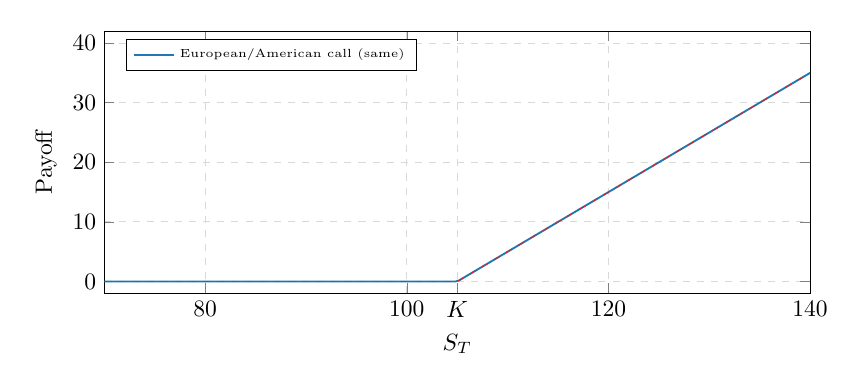
\begin{tikzpicture}[scale=0.85]
        \begin{axis}[
          xlabel={$S_T$}, ylabel={Payoff},
          xmin=70, xmax=140, ymin=-2, ymax=42,
          xtick={80,100,105,120,140},
          xticklabels={80,100,$K$,120,140},
          grid=major, grid style={dashed,gray!30},
          width=\textwidth, height=5.5cm,
          legend pos=north west, legend style={font=\tiny},
        ]
          \addplot[thick, color=euroblue, domain=70:140, samples=200]
            {max(x-105,0)};
          \addlegendentry{European/American call (same)}
          \addplot[dashed, color=amred, domain=70:140, samples=200]
            {max(x-105,0)};
        \end{axis}
      \end{tikzpicture}

    \column{0.48\textwidth}
      \centering\textbf{Put options}
      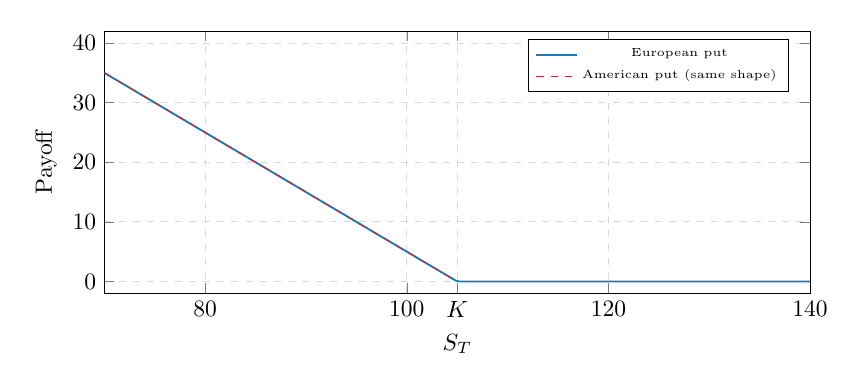
\begin{tikzpicture}[scale=0.85]
        \begin{axis}[
          xlabel={$S_T$}, ylabel={Payoff},
          xmin=70, xmax=140, ymin=-2, ymax=42,
          xtick={80,100,105,120,140},
          xticklabels={80,100,$K$,120,140},
          grid=major, grid style={dashed,gray!30},
          width=\textwidth, height=5.5cm,
          legend pos=north east, legend style={font=\tiny},
        ]
          \addplot[thick, color=euroblue, domain=70:140, samples=200]
            {max(105-x,0)};
          \addlegendentry{European put}
          \addplot[dashed, color=amred, domain=70:105, samples=200]
            {max(105-x,0)};
          \addlegendentry{American put (same shape)}
        \end{axis}
      \end{tikzpicture}
  \end{columns}

  \smallskip
  \centering
  \footnotesize
  The \emph{terminal} payoff is identical---the difference lies in
  \textbf{when} exercise is allowed.
\end{frame}

% ──────────────────────────────────────────────────────────────────────────────
\begin{frame}{Early Exercise and the Early-Exercise Premium}
  \begin{block}{When is early exercise optimal?}
    \begin{itemize}
      \item \textbf{American call} on a \emph{non-dividend-paying} stock:
            \highlight{never} optimal to exercise early $\Rightarrow$ equals
            the European call price.
      \item \textbf{American put}: early exercise can be optimal when the
            option is deep in-the-money.  Receiving $K-S$ now and investing
            at rate~$r$ can outweigh waiting.
    \end{itemize}
  \end{block}

  \bigskip
  \textbf{Early-exercise premium} $= C^{\text{Am}} - C^{\text{Eu}} \ge 0$

  \medskip
  Parameters: $S_0=100$, $K=105$, $T=1$, $r=5\%$, $\sigma=20\%$

  \medskip
  \begin{tabular}{lrrl}
    \toprule
    & European & American & Premium \\
    \midrule
    Call & 8.0214 & 8.0232 & $\approx 0$ (no dividends) \\
    Put  & 7.9004 & 8.7416 & \highlight{+0.8412} \\
    \bottomrule
  \end{tabular}
\end{frame}

% ══════════════════════════════════════════════════════════════════════════════
\section{Pricing Methods}
% ══════════════════════════════════════════════════════════════════════════════

\begin{frame}{Overview of Pricing Methods}
  \begin{tabular}{llll}
    \toprule
    Method & Option type & Complexity & Accuracy \\
    \midrule
    Black-Scholes formula    & European only  & $O(1)$       & Exact (GBM) \\
    Binomial tree (CRR)      & European \& American & $O(N^2)$ & Converges in $N$ \\
    Monte Carlo (plain)      & European \& exotic & $O(M)$ & $\pm 1/\sqrt{M}$ \\
    Longstaff-Schwartz (LSM) & American       & $O(M \cdot N)$ & $\pm 1/\sqrt{M}$ \\
    \bottomrule
  \end{tabular}

  \bigskip
  \begin{itemize}
    \item $N$ = number of time steps, $M$ = number of Monte Carlo paths
    \item This library implements \textbf{all four} methods
    \item Black-Scholes and binomial trees serve as \textbf{benchmarks} for
          validating Monte Carlo results
  \end{itemize}
\end{frame}

% ══════════════════════════════════════════════════════════════════════════════
\section{Black-Scholes (European)}
% ══════════════════════════════════════════════════════════════════════════════

\begin{frame}{Black-Scholes Model}
  Under the \textbf{risk-neutral measure}, stock prices follow GBM:
  \[
    dS = r S\,dt + \sigma S\,dW^{\Q}
  \]

  \begin{block}{Closed-form prices}
    \[
      C = S_0 \Phi(d_1) - K e^{-rT} \Phi(d_2), \qquad
      P = K e^{-rT} \Phi(-d_2) - S_0 \Phi(-d_1)
    \]
    \[
      d_1 = \frac{\ln(S_0/K) + (r + \tfrac{1}{2}\sigma^2)T}{\sigma\sqrt{T}},
      \qquad d_2 = d_1 - \sigma\sqrt{T}
    \]
  \end{block}

  \bigskip
  \textbf{Key properties}
  \begin{itemize}
    \item Put-call parity: $C - P = S_0 - K e^{-rT}$
    \item Only applies to \highlight{European} options on non-dividend-paying stocks
    \item Benchmark for Monte Carlo validation
  \end{itemize}
\end{frame}

% ──────────────────────────────────────────────────────────────────────────────
\begin{frame}{Black-Scholes: Numerical Example}
  Parameters: $S_0=100$, $K=105$, $T=1$\,yr, $r=5\%$, $\sigma=20\%$

  \bigskip
  \begin{columns}[T]
    \column{0.45\textwidth}
      \textbf{Calculation}
      \begin{align*}
        d_1 &= \frac{\ln(100/105)+(0.05+0.02)}{0.20} = 0.0217\\
        d_2 &= 0.0217 - 0.20 = -0.1783\\
        \Phi(d_1) &= 0.5087,\quad \Phi(d_2) = 0.4292\\[4pt]
        C &= 100(0.5087) - 105 e^{-0.05}(0.4292) \\
          &= \mathbf{8.0214}\\[4pt]
        P &= 105 e^{-0.05}(0.5708) - 100(0.4913) \\
          &= \mathbf{7.9004}
      \end{align*}

    \column{0.52\textwidth}
      \textbf{Put-call parity check}
      \[
        C - P = 8.0214 - 7.9004 = 0.1210
      \]
      \[
        S_0 - Ke^{-rT} = 100 - 105 e^{-0.05} = 0.1209\;\checkmark
      \]
      \bigskip
      \textbf{Monte Carlo validation}\\[4pt]
      \begin{tabular}{lrr}
        \toprule
        & MC price & BS price \\
        \midrule
        Call & 8.0398 & 8.0214 \\
        Put  & 7.9214 & 7.9004 \\
        \bottomrule
      \end{tabular}\\[4pt]
      \footnotesize (200k paths, SE $\approx 0.03$)
  \end{columns}
\end{frame}

% ══════════════════════════════════════════════════════════════════════════════
\section{Monte Carlo Simulation}
% ══════════════════════════════════════════════════════════════════════════════

\begin{frame}{Monte Carlo Pricing (European Options)}
  \textbf{Algorithm}
  \begin{enumerate}
    \item Simulate $M$ terminal stock prices under $\Q$:
          \[
            S_T^{(i)} = S_0 \exp\!\Bigl[\bigl(r - \tfrac{\sigma^2}{2}\bigr)T
                         + \sigma\sqrt{T}\,Z^{(i)}\Bigr],\quad Z^{(i)}\sim\mathcal{N}(0,1)
          \]
    \item Compute payoffs: $h^{(i)} = \max(S_T^{(i)} - K,\,0)$
    \item Estimate price: $\hat{C} = e^{-rT}\,\dfrac{1}{M}\sum_{i=1}^{M} h^{(i)}$
  \end{enumerate}

  \bigskip
  \textbf{Standard error} scales as $1/\sqrt{M}$: doubling accuracy costs 4$\times$ more paths.

  \begin{block}{Variance reduction: antithetic variates}
    For each $Z^{(i)}$, also simulate with $-Z^{(i)}$.  Average the paired payoffs
    to cancel common noise.  In practice: \highlight{$\sim$1.26$\times$ SE reduction}
    (free, no extra simulations).
  \end{block}
\end{frame}

% ──────────────────────────────────────────────────────────────────────────────
\begin{frame}{Monte Carlo: Standard Error vs.\ Path Count}
  \begin{columns}[T]
    \column{0.5\textwidth}
      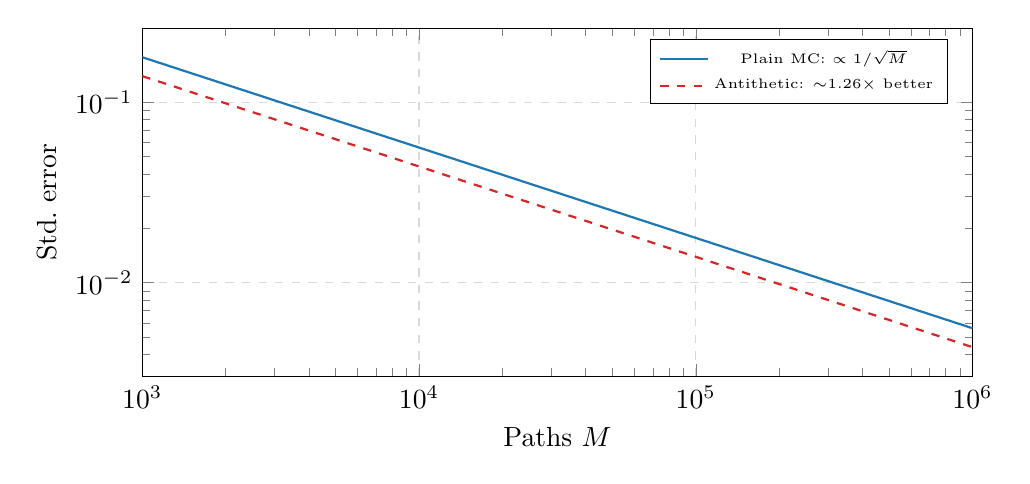
\begin{tikzpicture}
        \begin{axis}[
          xlabel={Paths $M$}, ylabel={Std.\ error},
          xmode=log, ymode=log,
          xmin=1000, xmax=1000000,
          grid=major, grid style={dashed,gray!30},
          width=\textwidth, height=6cm,
          legend pos=north east, legend style={font=\tiny},
        ]
          % SE ~ sigma/sqrt(M), sigma ~ 8 * 0.7 ~ 5.6 for call payoffs
          \addplot[thick, color=euroblue, domain=1000:1000000, samples=50]
            {5.6/sqrt(x)};
          \addlegendentry{Plain MC: $\propto 1/\sqrt{M}$}
          \addplot[thick, dashed, color=amred, domain=1000:1000000, samples=50]
            {4.4/sqrt(x)};
          \addlegendentry{Antithetic: $\sim$1.26$\times$ better}
        \end{axis}
      \end{tikzpicture}

    \column{0.48\textwidth}
      \textbf{European call, $K=105$, $T=1$yr}

      \medskip
      \begin{tabular}{rrc}
        \toprule
        Paths & Std.\ error & 95\% CI width \\
        \midrule
        10{,}000   & 0.054 & $\pm$0.11 \\
        50{,}000   & 0.024 & $\pm$0.05 \\
        100{,}000  & 0.017 & $\pm$0.03 \\
        200{,}000  & 0.012 & $\pm$0.02 \\
        1{,}000{,}000 & 0.005 & $\pm$0.01 \\
        \bottomrule
      \end{tabular}

      \medskip
      \footnotesize Antithetic variates (200k paths):
      SE = 0.0236 vs.\ 0.0297 plain.
  \end{columns}
\end{frame}

% ══════════════════════════════════════════════════════════════════════════════
\section{American Option Pricing}
% ══════════════════════════════════════════════════════════════════════════════

\begin{frame}{CRR Binomial Tree (American Options)}
  \textbf{Setup} (Cox-Ross-Rubinstein, 1979)

  Divide $[0,T]$ into $N$ steps of size $\Delta t = T/N$:
  \[
    u = e^{\sigma\sqrt{\Delta t}},\quad d = 1/u,\quad
    p = \frac{e^{r\Delta t} - d}{u - d}
  \]

  \begin{columns}[T]
    \column{0.48\textwidth}
      \textbf{Algorithm}
      \begin{enumerate}
        \item Build terminal node prices $S_0\,u^j\,d^{N-j}$
        \item Set terminal values $V_j = \max(K - S_j, 0)$
        \item Roll back:
              \[
                V_j = e^{-r\Delta t}(p\,V_j + (1-p)\,V_{j+1})
              \]
        \item Apply early-exercise:
              \[
                V_j \leftarrow \max(V_j,\; K - S_j)
              \]
      \end{enumerate}

    \column{0.48\textwidth}
      \textbf{Convergence} (American put, $K=105$)

      \medskip
      \begin{tabular}{rc}
        \toprule
        Steps $N$ & Price \\
        \midrule
        10  & 8.8550 \\
        50  & 8.7357 \\
        100 & 8.7476 \\
        200 & 8.7436 \\
        500 & \textbf{8.7416} \\
        \bottomrule
      \end{tabular}

      \medskip
      \footnotesize Converges to $\approx8.742$ well before $N=500$.
  \end{columns}
\end{frame}

% ──────────────────────────────────────────────────────────────────────────────
\begin{frame}{Longstaff-Schwartz (LSM) Algorithm}
  \textbf{Key idea}: use least-squares regression to estimate the
  \emph{continuation value} at each exercise date.

  \bigskip
  \textbf{Algorithm} \small(Longstaff \& Schwartz, RFS 2001)
  \begin{enumerate}
    \item Simulate $M$ full price paths $\{S_t^{(i)}\}$, $t=0,\Delta t,\ldots,T$
    \item Initialise $V^{(i)} = \max(K - S_T^{(i)}, 0)$ (terminal payoff)
    \item \textbf{Backward induction}: for $t = T-\Delta t, \ldots, \Delta t$:
      \begin{enumerate}
        \item Discount: $V^{(i)} \leftarrow e^{-r\Delta t}\,V^{(i)}$
        \item For in-the-money paths, regress $V^{(i)}$ on
              $\bigl[1,\,S_t^{(i)},\,(S_t^{(i)})^2\bigr]$
              to estimate the continuation value $\hat{C}(S_t^{(i)})$
        \item If $\max(K - S_t^{(i)},0) > \hat{C}(S_t^{(i)})$: exercise early,
              set $V^{(i)} = K - S_t^{(i)}$
      \end{enumerate}
    \item Price $= e^{-r\Delta t}\,\E[V]$
  \end{enumerate}
\end{frame}

% ──────────────────────────────────────────────────────────────────────────────
\begin{frame}[fragile]{LSM: Code Sketch}
\begin{lstlisting}[language=Python]
# Simulate M paths with N steps
paths = simulator.simulate_paths(T, N, M, risk_neutral=True)

# Terminal payoff
V = np.maximum(K - paths[:, -1], 0.0)

# Backward induction
for step in range(N-1, 0, -1):
    V *= discount               # discount one period
    S = paths[:, step]
    intrinsic = np.maximum(K - S, 0.0)
    itm = intrinsic > 0         # in-the-money mask

    # Least-squares regression on ITM paths
    X = np.column_stack([np.ones(itm.sum()), S[itm], S[itm]**2])
    coeffs, *_ = np.linalg.lstsq(X, V[itm], rcond=None)
    continuation = X @ coeffs

    # Early exercise where intrinsic beats continuation
    exercise = intrinsic[itm] > continuation
    V[np.where(itm)[0][exercise]] = intrinsic[itm][exercise]

V *= discount                   # discount to t=0
price = V.mean()
\end{lstlisting}
\end{frame}

% ══════════════════════════════════════════════════════════════════════════════
\section{Numerical Examples and Benchmarking}
% ══════════════════════════════════════════════════════════════════════════════

\begin{frame}{Numerical Results: All Methods}
  Parameters: $S_0=100$, $K=105$, $T=1$\,yr, $r=5\%$, $\sigma=20\%$

  \bigskip
  \begin{tabular}{llccc}
    \toprule
    Option & Method & Price & Std.\ error & vs.\ benchmark \\
    \midrule
    European call & Black-Scholes   & 8.0214 & exact    & --- \\
                  & Monte Carlo     & 8.0398 & 0.0297   & $+0.018$ \\
                  & Antithetic MC   & 8.0461 & 0.0236   & $+0.025$ \\
    \midrule
    European put  & Black-Scholes   & 7.9004 & exact    & --- \\
                  & Monte Carlo     & 7.9214 & 0.0232   & $+0.021$ \\
    \midrule
    American call & Binomial ($N=500$) & 8.0232 & ---   & --- \\
                  & LSM ($M=200$k)  & 8.0113 & 0.0294   & $-0.012$ \\
    \midrule
    American put  & Binomial ($N=500$) & 8.7416 & ---   & --- \\
                  & LSM ($M=200$k)  & 8.6972 & 0.0182   & $-0.044$ \\
    \bottomrule
  \end{tabular}

  \medskip
  \footnotesize All MC differences lie within $\sim$2 standard errors of the benchmark.
\end{frame}

% ──────────────────────────────────────────────────────────────────────────────
\begin{frame}{Early-Exercise Premium vs.\ Moneyness}
  American put premium $= C^{\text{Am}}_{\text{put}} - C^{\text{Eu}}_{\text{put}}$
  as a function of spot price ($K=105$, $T=1$yr, $r=5\%$, $\sigma=20\%$)

  \begin{columns}[T]
    \column{0.52\textwidth}
      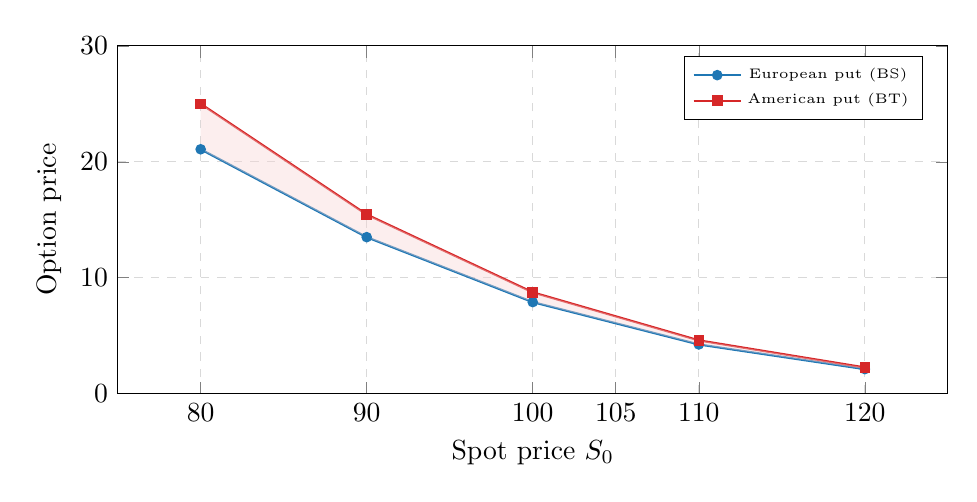
\begin{tikzpicture}
        \begin{axis}[
          xlabel={Spot price $S_0$},
          ylabel={Option price},
          xmin=75, xmax=125,
          ymin=0, ymax=30,
          grid=major, grid style={dashed,gray!30},
          width=\textwidth, height=6cm,
          legend pos=north east, legend style={font=\tiny},
          xtick={80,90,100,105,110,120},
        ]
          % European put (BS)
          \addplot[thick, color=euroblue, mark=*, mark size=1.5pt]
            coordinates {(80,21.079)(90,13.500)(100,7.900)(110,4.249)(120,2.122)};
          \addlegendentry{European put (BS)}
          % American put (BT)
          \addplot[thick, color=amred, mark=square*, mark size=1.5pt]
            coordinates {(80,25.000)(90,15.454)(100,8.742)(110,4.600)(120,2.263)};
          \addlegendentry{American put (BT)}
          % Premium shading (approximate)
          \addplot[fill=amred!20, opacity=0.4, draw=none]
            coordinates {(80,21.079)(90,13.500)(100,7.900)(110,4.249)(120,2.122)
                         (120,2.263)(110,4.600)(100,8.742)(90,15.454)(80,25.000)};
        \end{axis}
      \end{tikzpicture}

    \column{0.46\textwidth}
      \begin{tabular}{rccc}
        \toprule
        $S_0$ & EU put & AM put & Premium \\
        \midrule
        80  & 21.079 & \textbf{25.000} & \highlight{3.921} \\
        90  & 13.500 & 15.454 & 1.954 \\
        100 & 7.900  & 8.742  & 0.841 \\
        110 & 4.249  & 4.600  & 0.351 \\
        120 & 2.122  & 2.263  & 0.141 \\
        \bottomrule
      \end{tabular}

      \bigskip
      \footnotesize
      Premium is largest when the option is \textbf{deep in-the-money}:
      immediate exercise yields $K-S_0$ cash now, which earns interest.
      At $S_0=80$, the American put equals its intrinsic value
      $K-S_0=25$ (immediate exercise is optimal).
  \end{columns}
\end{frame}

% ──────────────────────────────────────────────────────────────────────────────
\begin{frame}{Benchmarking: LSM vs.\ Binomial Tree}
  \begin{columns}[T]
    \column{0.5\textwidth}
      \textbf{American put} ($S_0=100$, $K=105$, $T=1$yr)

      \medskip
      \begin{tabular}{lrc}
        \toprule
        Method & Price & Error \\
        \midrule
        BT $N=500$ (ref.)  & 8.7416 & --- \\
        BT $N=10$           & 8.8550 & $+0.113$ \\
        BT $N=50$           & 8.7357 & $-0.006$ \\
        BT $N=100$          & 8.7476 & $+0.006$ \\
        BT $N=200$          & 8.7436 & $+0.002$ \\
        \midrule
        LSM $M=50$k  & 8.71   & $-0.03$ \\
        LSM $M=100$k & 8.72   & $-0.02$ \\
        LSM $M=200$k & 8.6972 & $-0.044$ \\
        \bottomrule
      \end{tabular}

    \column{0.48\textwidth}
      \textbf{Observations}
      \begin{itemize}
        \item Binomial tree converges quickly; $N=50$ is already accurate
              to $< 0.01$
        \item LSM is a \highlight{lower bound}: regression underestimates
              continuation value, triggering slightly too much early exercise
        \item Both methods agree to within $\pm 0.05$ — well within
              Monte Carlo standard error ($\sim 0.02$--$0.03$)
        \item Binomial tree is fast for single options; LSM scales to
              \textbf{path-dependent} and \textbf{multi-asset} settings
              where trees are infeasible
      \end{itemize}
  \end{columns}
\end{frame}

% ══════════════════════════════════════════════════════════════════════════════
\section{Summary}
% ══════════════════════════════════════════════════════════════════════════════

\begin{frame}{Summary}
  \begin{columns}[T]
    \column{0.48\textwidth}
      \textbf{Key takeaways}
      \begin{itemize}
        \item European options: exercisable only at $T$;
              priced exactly by \textbf{Black-Scholes}
        \item American options: exercisable at any $t \le T$;
              always $\ge$ European counterpart
        \item American call $\approx$ European call (no dividends)
        \item American put carries a meaningful
              \highlight{early-exercise premium}, largest when deep ITM
        \item \textbf{LSM} extends Monte Carlo to American options
              via regression-based continuation value estimation
        \item \textbf{Binomial trees} give fast, accurate benchmarks
              for vanilla American options
      \end{itemize}

    \column{0.48\textwidth}
      \textbf{Method comparison}

      \medskip
      \begin{tabular}{lcc}
        \toprule
        & European & American \\
        \midrule
        Analytical  & BS & --- \\
        Tree        & CRR & CRR + EE \\
        Monte Carlo & Plain MC & LSM \\
        \bottomrule
      \end{tabular}

      \bigskip
      \textbf{This library}
      \begin{itemize}
        \item \texttt{engine.price()} — European / exotic
        \item \texttt{engine.price\_american()} — LSM
        \item \texttt{black\_scholes\_call/put} — BS benchmark
        \item \texttt{binomial\_tree\_american\_*} — tree benchmark
      \end{itemize}
  \end{columns}
\end{frame}

% ──────────────────────────────────────────────────────────────────────────────
\begin{frame}[plain]
  \begin{center}
    \Large\textbf{Thank you}
  \end{center}
\end{frame}

\end{document}
